\chapter{Zadatak D} \label{ch:d}

U ovom poglavlju je opisan i odrađen zadatak D.

\section{Opis zadatka} \label{sec:d:opis}
odrediti svaku komponentu mehaničke snage potrebne za savladavanje otpora na temelju fizikalne
slike vozila. Potrebno je prikazati krivulje svake komponente mehaničke snage zasebno i sve na
jednom grafu s točno naznačenim oznakama. Dodatno, za svaku komponentu snage je potrebno
odrediti minimalnu, maksimalnu i srednju vrijednost krivulje, te prikazati je u tabličnom obliku.

\section{Rješenje} \label{sec:d:rjesenje}

Za riješavanje ovog zadatka potrebno je izračunati pomnožiti sve sile iz zadatka c sa brzinom vozila.
Brzinu vozila je potrebno podijeliti s 3.6 pošto je mjerena u km/h.


\begin{figure}
    \centering
    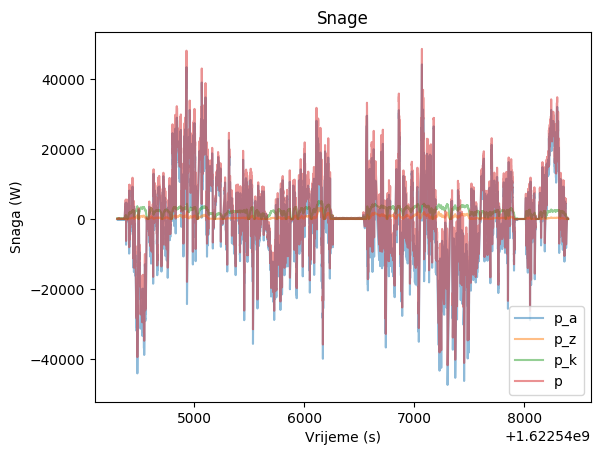
\includegraphics[width=0.8\textwidth]{images/powers.png}
    \caption{Prikaz izračunate snage kroz vrijeme.}
    \label{fig:d:power_graph}
\end{figure}


\begin{table}[!ht]
    \centering
    \caption{Anaiza snaga na vozilu}
    \begin{tabular}{lllll}
    \hline
        \textbf{describe} & \textbf{p\_a} & \textbf{p\_z} & \textbf{p\_k} & \textbf{p} \\ \hline
        count & 9776.0 & 9776.0 & 9776.0 & 9776.0 \\ 
        null\_count & 0.0 & 0.0 & 0.0 & 0.0 \\ 
        mean & 516.75318 & 414.467539 & 1876.065364 & 2807.286083 \\ 
        std & 10284.685553 & 520.405078 & 1315.56626 & 10458.743532 \\ 
        min & -47349.443215 & 0.0 & 0.0 & -41737.887992 \\ 
        25\% & -4092.952681 & 0.256285 & 216.047435 & -1485.0432 \\ 
        50\% & 58.491354 & 245.45779 & 2122.481816 & 252.956319 \\ 
        75\% & 5408.477454 & 671.446613 & 2962.317587 & 8141.98921 \\ 
        max & 44103.738373 & 3118.223036 & 5060.441445 & 48529.830356 \\ \hline
    \end{tabular}
    \label{table:c:powers}
\end{table}